% Content for DWT Results subsection
% This file is included in the main conference paper via % Content for DWT Results subsection
% This file is included in the main conference paper via % Content for DWT Results subsection
% This file is included in the main conference paper via % Content for DWT Results subsection
% This file is included in the main conference paper via \input{DWTResults}

\begin{figure}[ht]
  \centering
  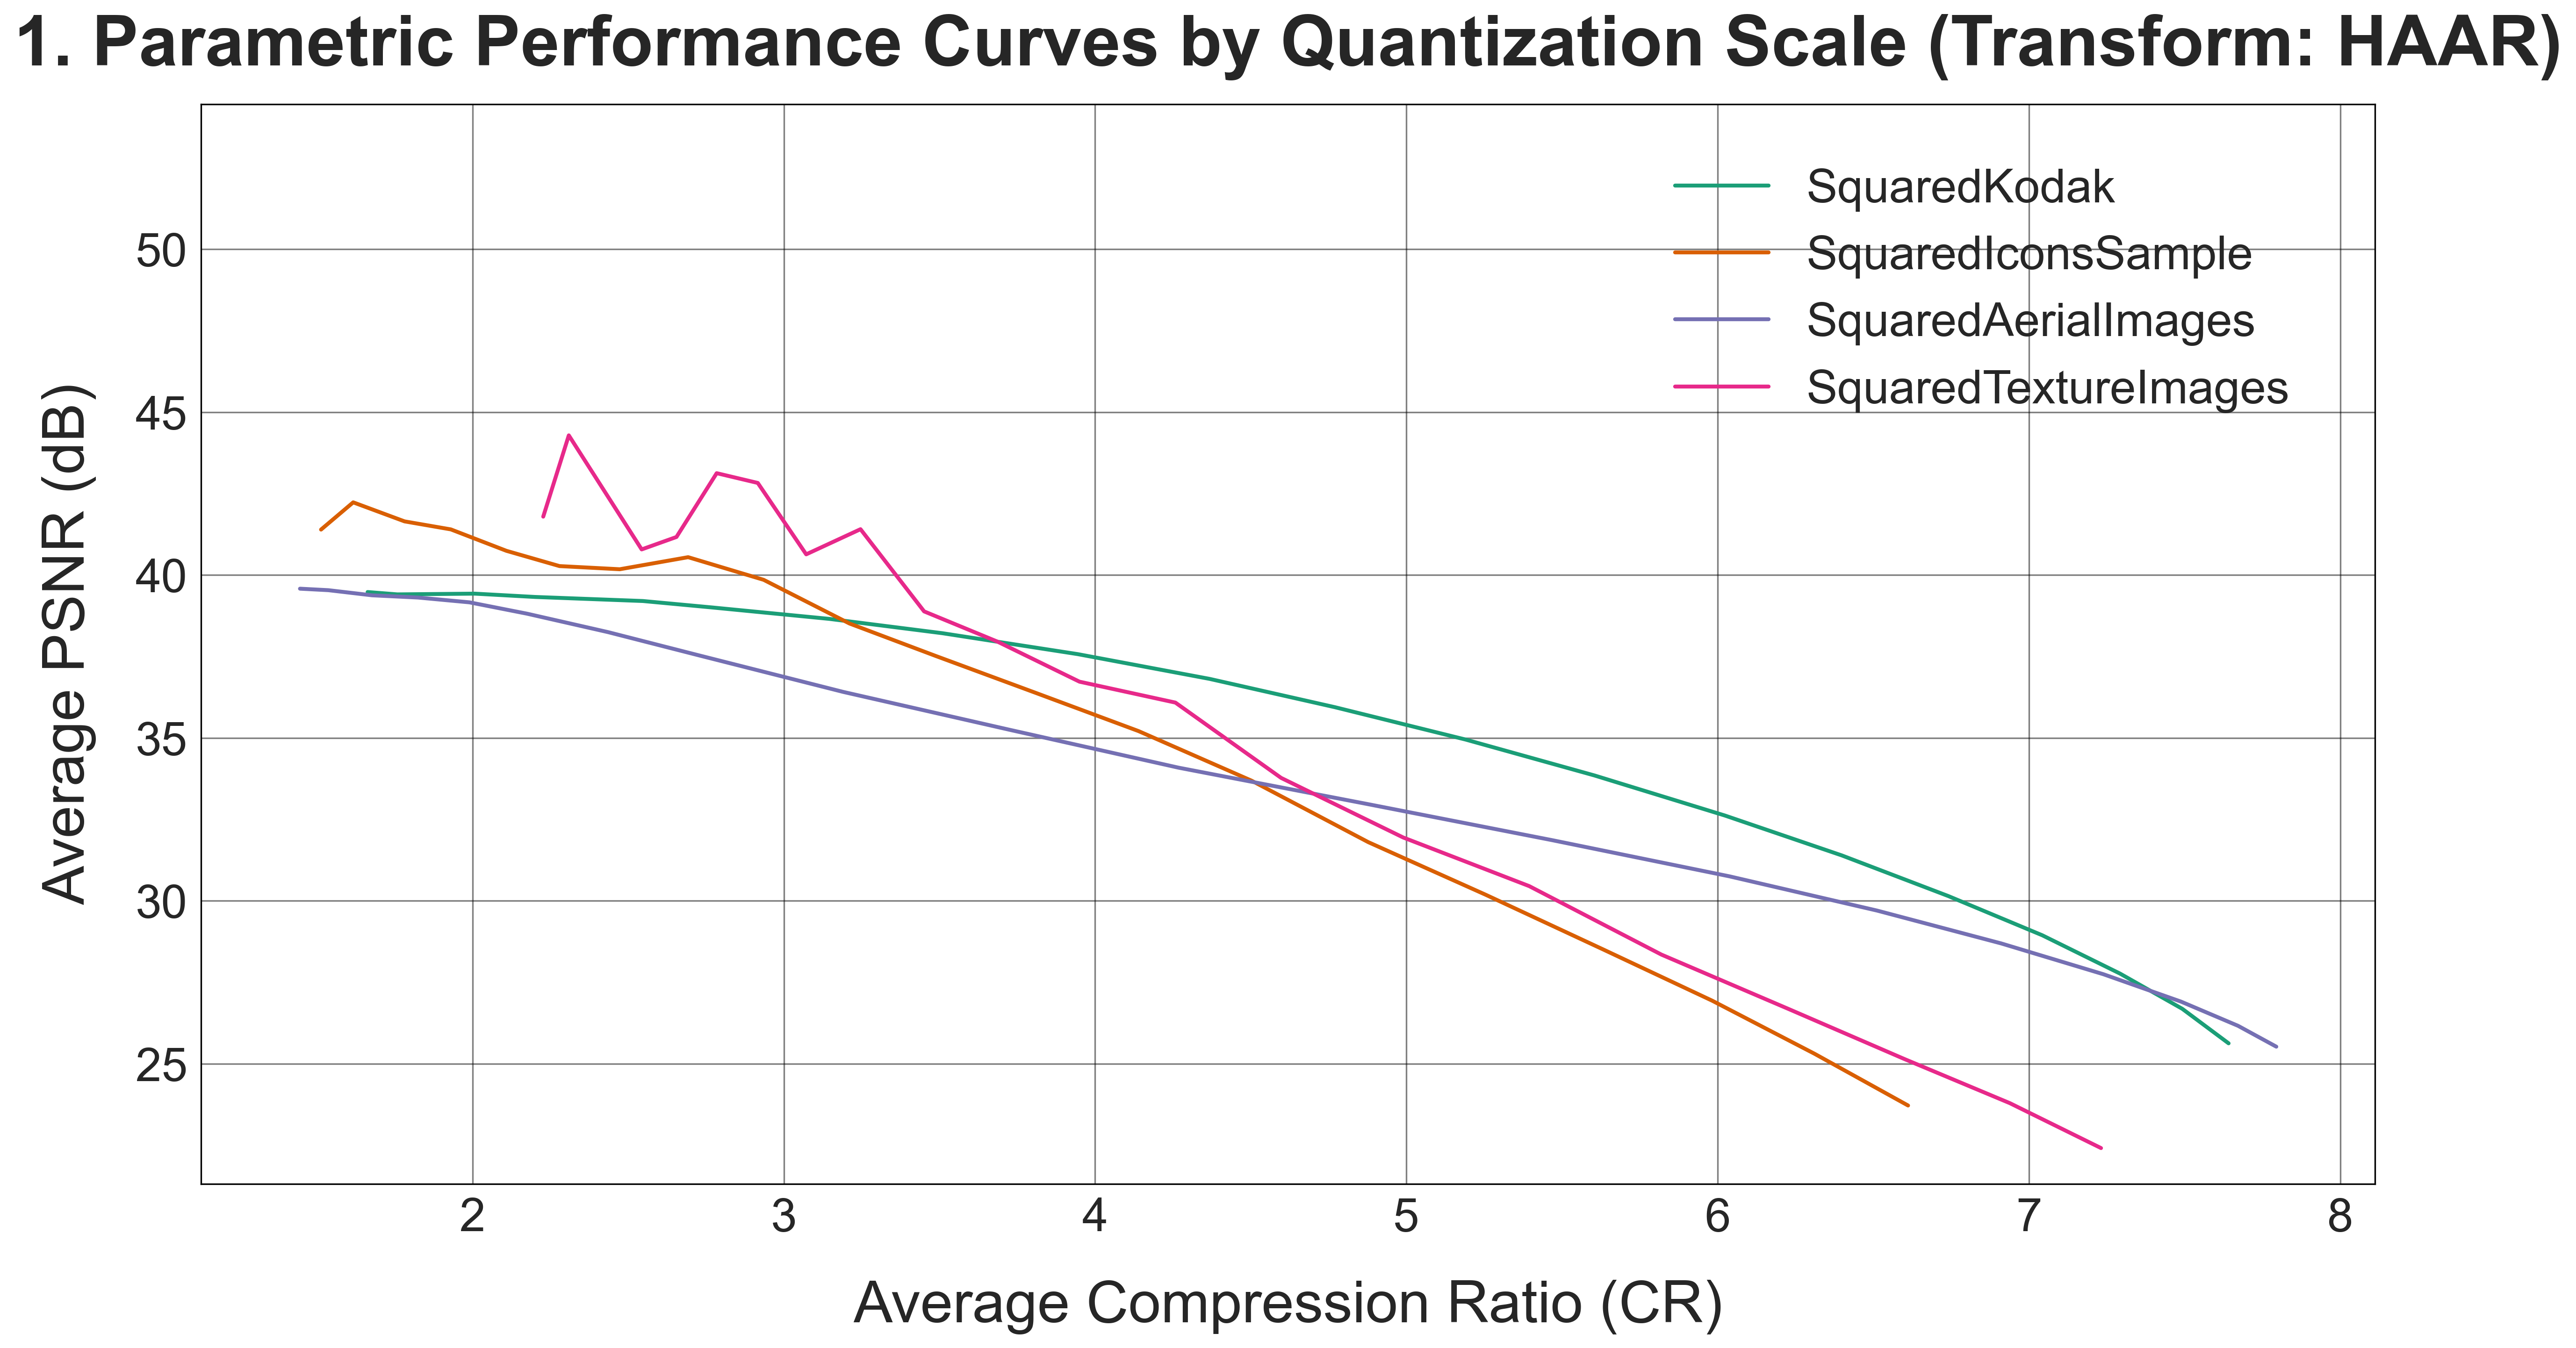
\includegraphics[width=0.48\textwidth]{results/plots/plot_1_parametric_curve_HAAR.png}
  \caption{Performance of the Haar wavelet transform across different datasets}
  \label{fig:dwt_results}
\end{figure}

The results demonstrate that the Discrete Wavelet Transform (DWT) using the Haar wavelet basis exhibits varying performance across different image datasets. Notably, the method performed worse on the Texture Images and Icons Images datasets as quantization became more aggressive compared to other image types as can be see in Figure~\ref{fig:dwt_results}.

\begin{figure}[ht]
  \centering
  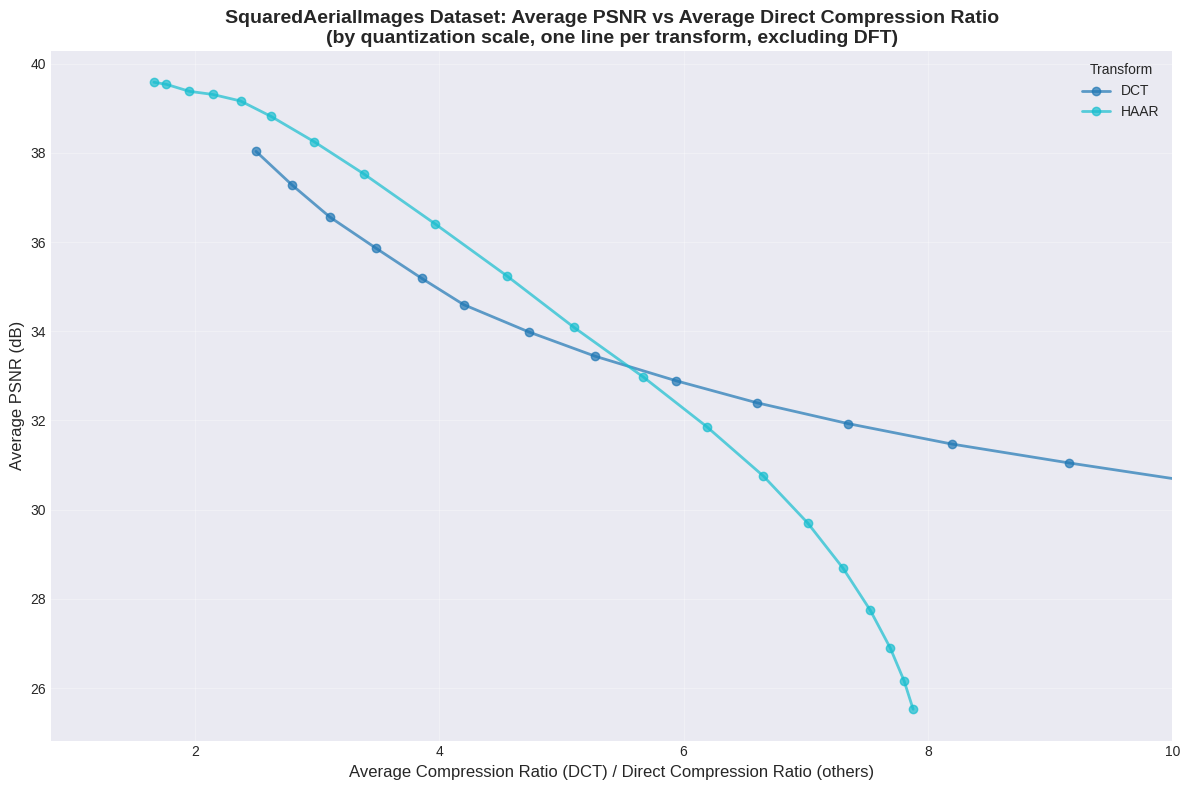
\includegraphics[width=0.48\textwidth]{results/plots/parametric_aerial.png}
  \caption{Performance comparison of Haar and DCT on aerial images.}
  \label{fig:dwt_aerial}
\end{figure}

Figure~\ref{fig:dwt_aerial} shows that the Haar wavelet transform performs slightly better than DCT on aerial images at smaller compression ratios.

\begin{figure}[ht]
  \centering
  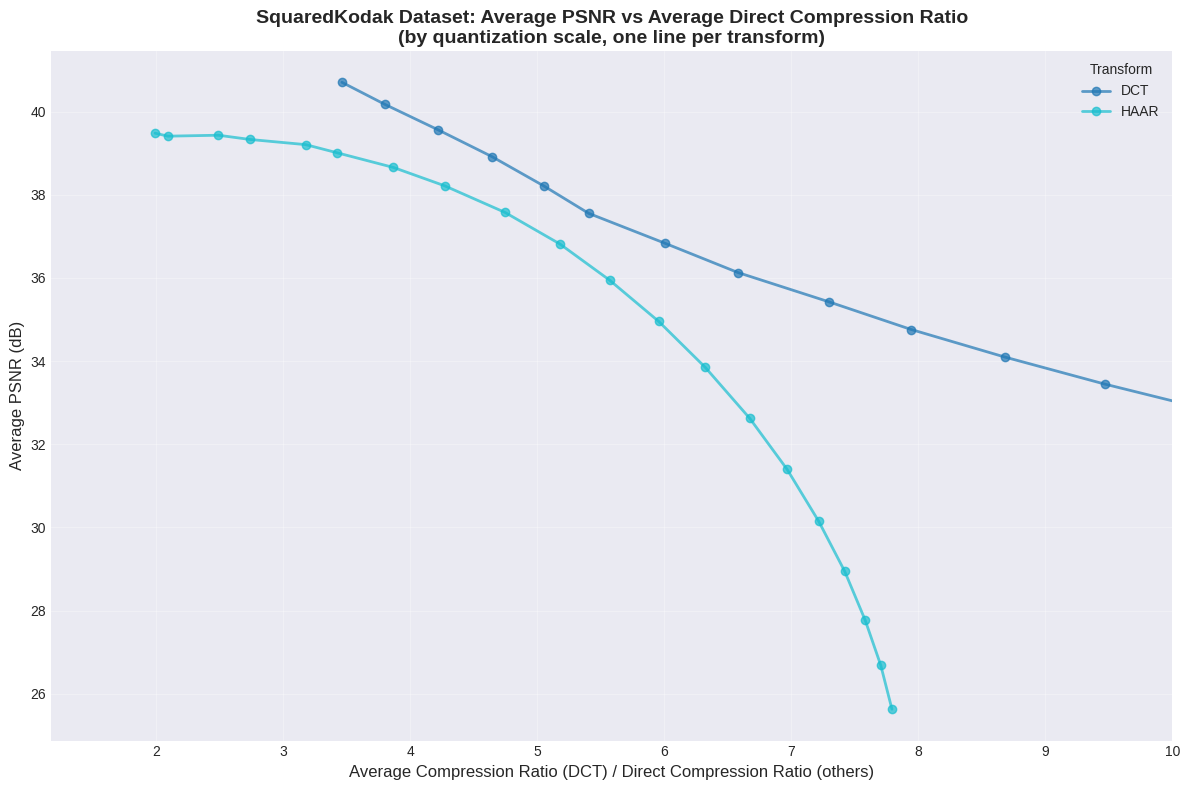
\includegraphics[width=0.48\textwidth]{results/plots/parametric_kodak.png}
  \caption{Performance comparison of Haar and DCT on Kodak images.}
  \label{fig:dwt_kodak}
\end{figure}

In contrast, Figure~\ref{fig:dwt_kodak} demonstrates that Haar performs worse than DCT on Kodak images across all compression ratio scenarios.


\begin{figure}[ht]
  \centering
  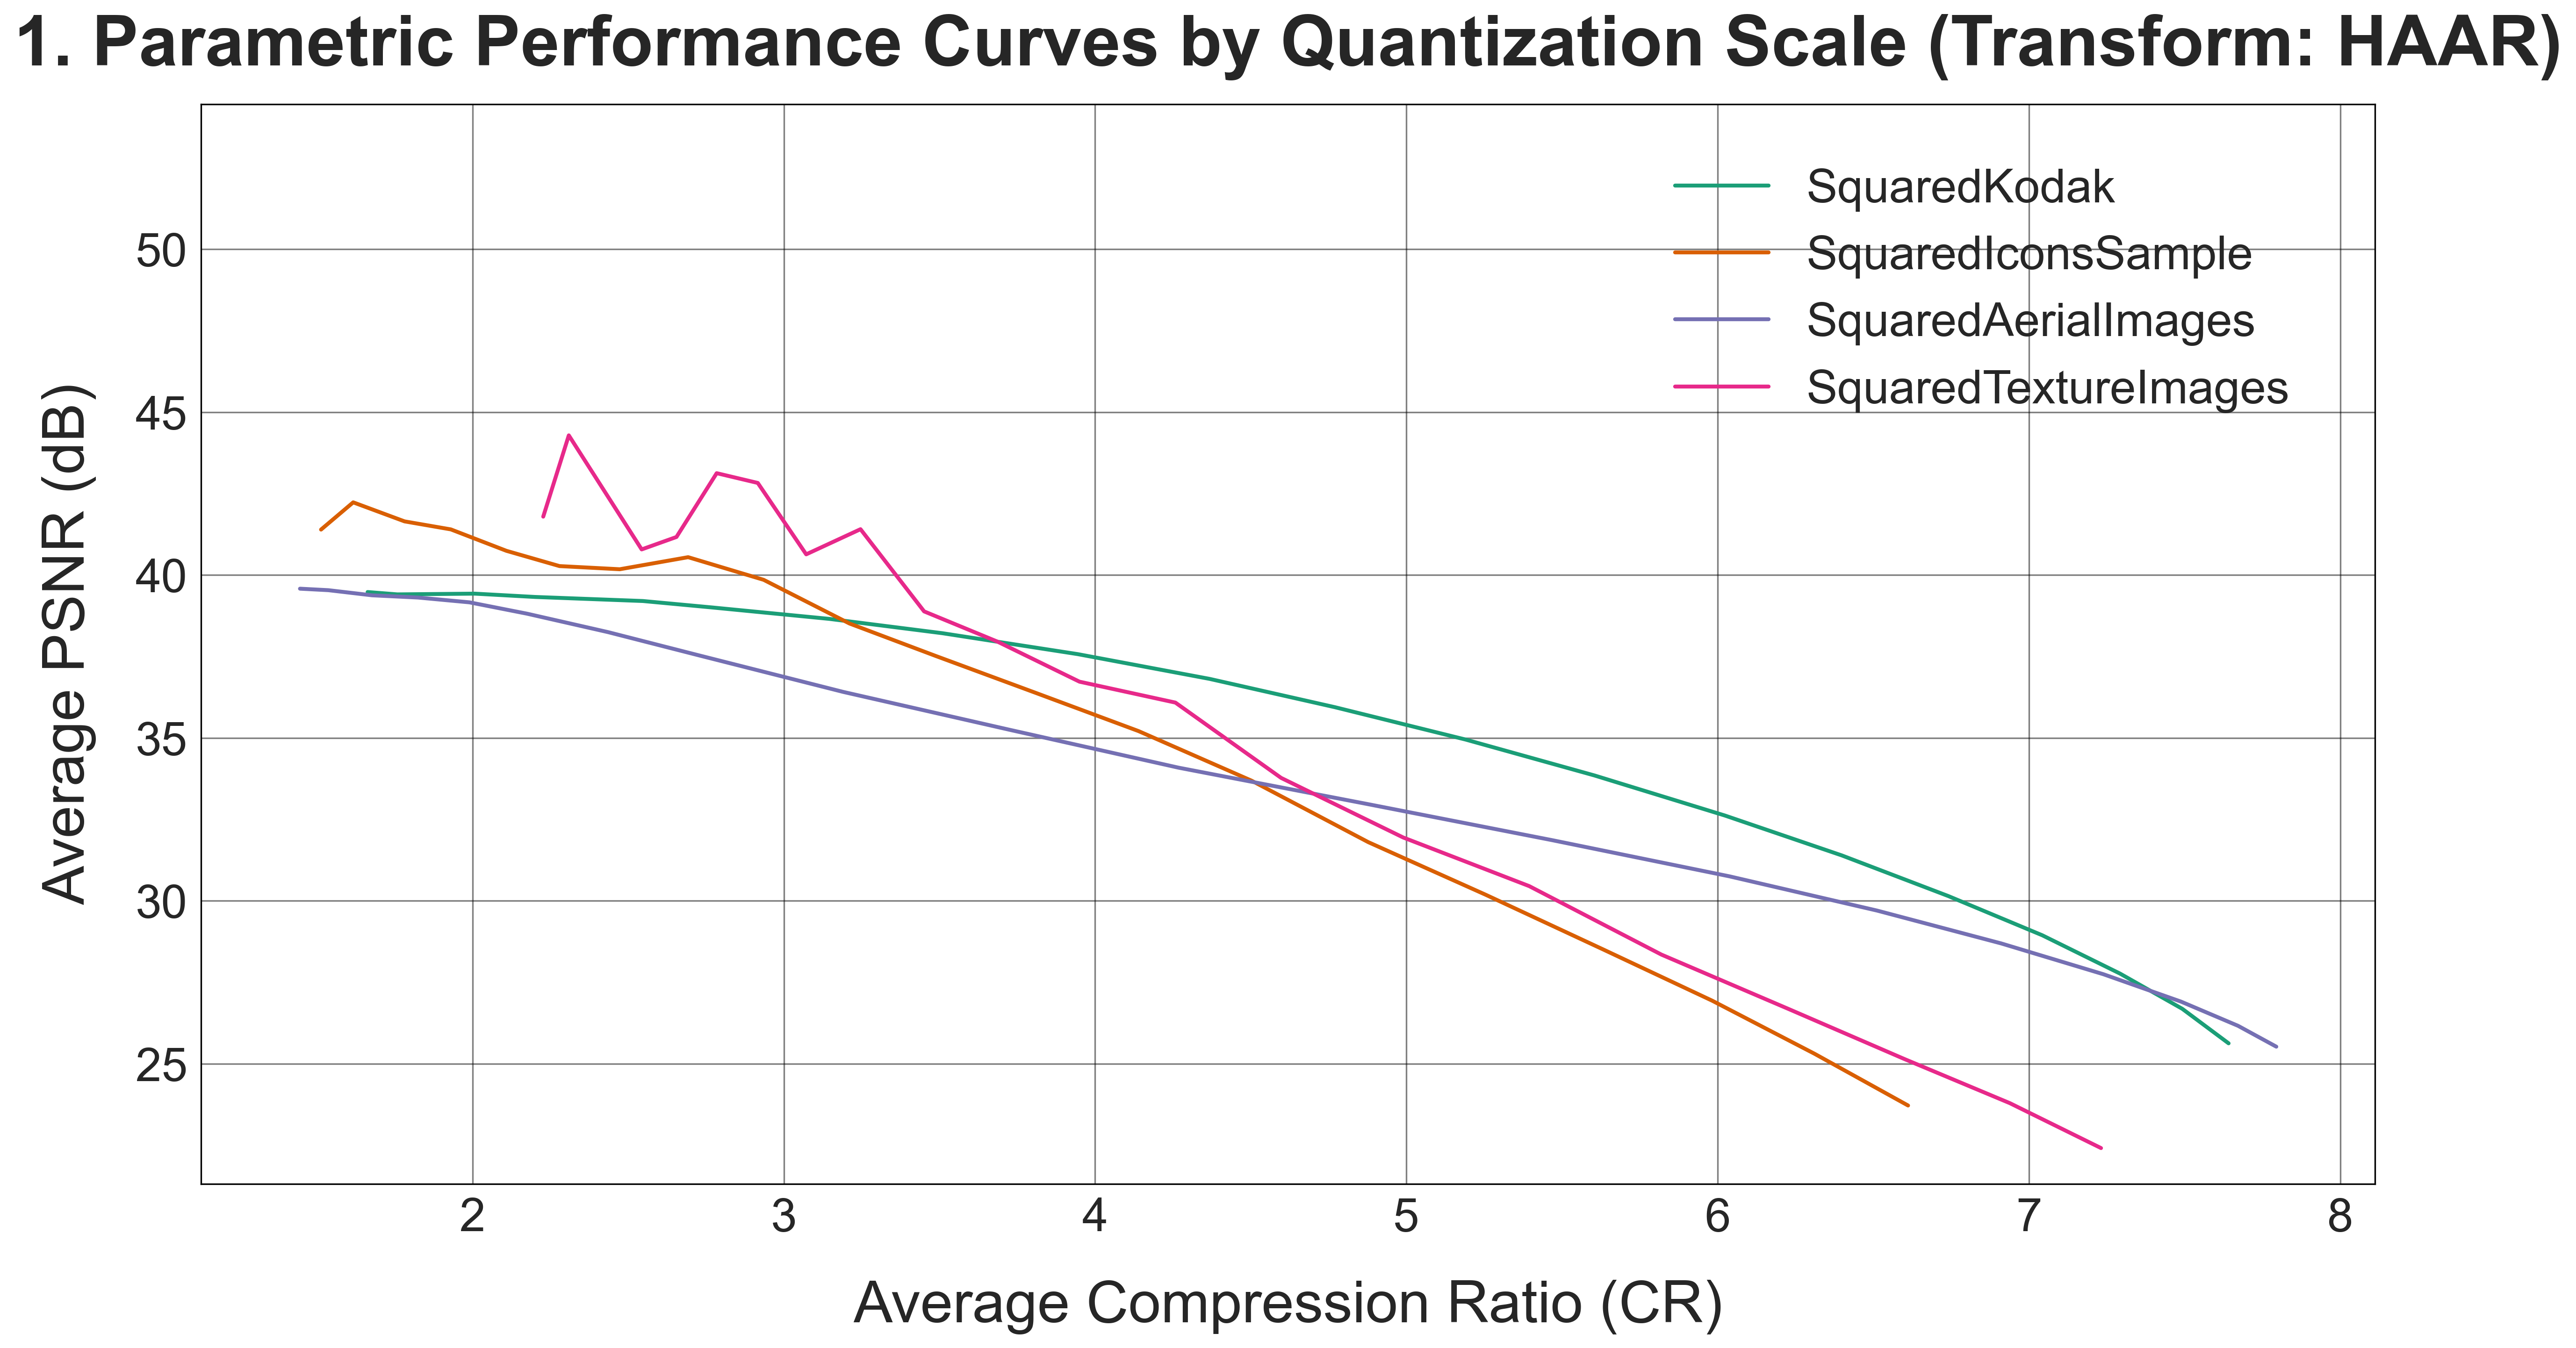
\includegraphics[width=0.48\textwidth]{results/plots/plot_1_parametric_curve_HAAR.png}
  \caption{Performance of the Haar wavelet transform across different datasets}
  \label{fig:dwt_results}
\end{figure}

The results demonstrate that the Discrete Wavelet Transform (DWT) using the Haar wavelet basis exhibits varying performance across different image datasets. Notably, the method performed worse on the Texture Images and Icons Images datasets as quantization became more aggressive compared to other image types as can be see in Figure~\ref{fig:dwt_results}.

\begin{figure}[ht]
  \centering
  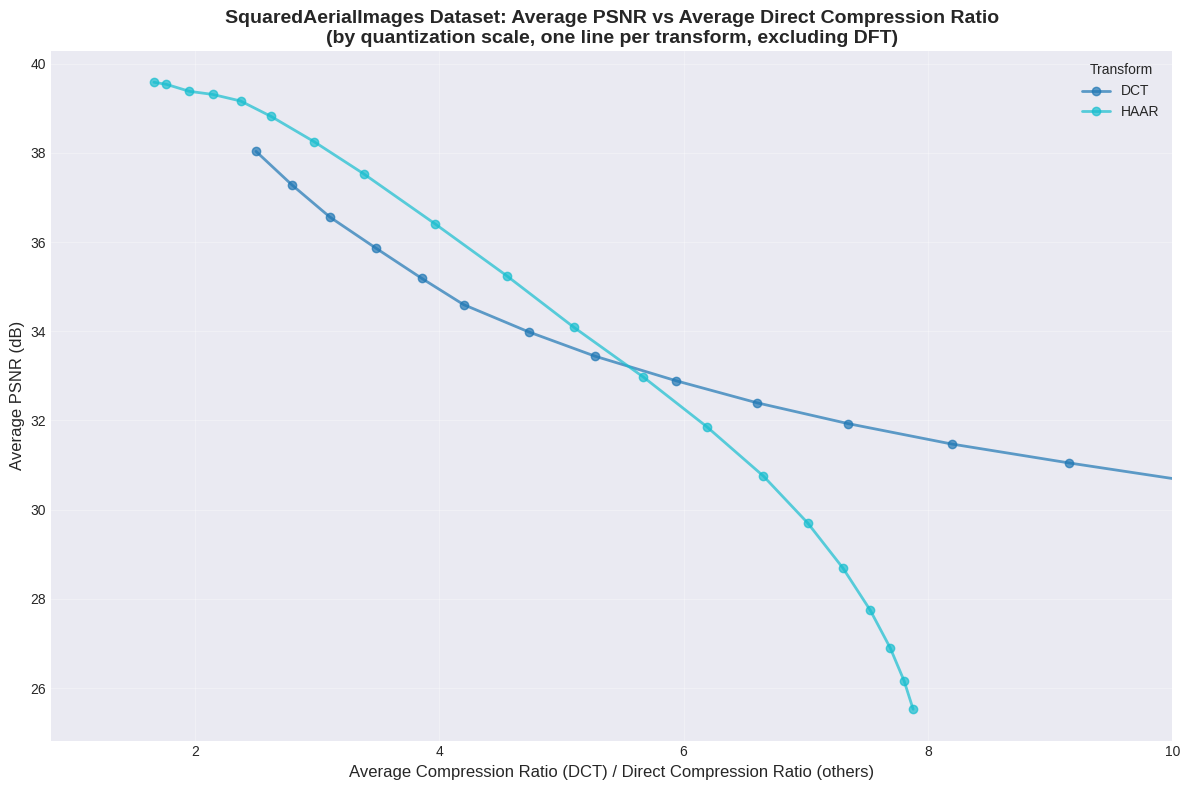
\includegraphics[width=0.48\textwidth]{results/plots/parametric_aerial.png}
  \caption{Performance comparison of Haar and DCT on aerial images.}
  \label{fig:dwt_aerial}
\end{figure}

Figure~\ref{fig:dwt_aerial} shows that the Haar wavelet transform performs slightly better than DCT on aerial images at smaller compression ratios.

\begin{figure}[ht]
  \centering
  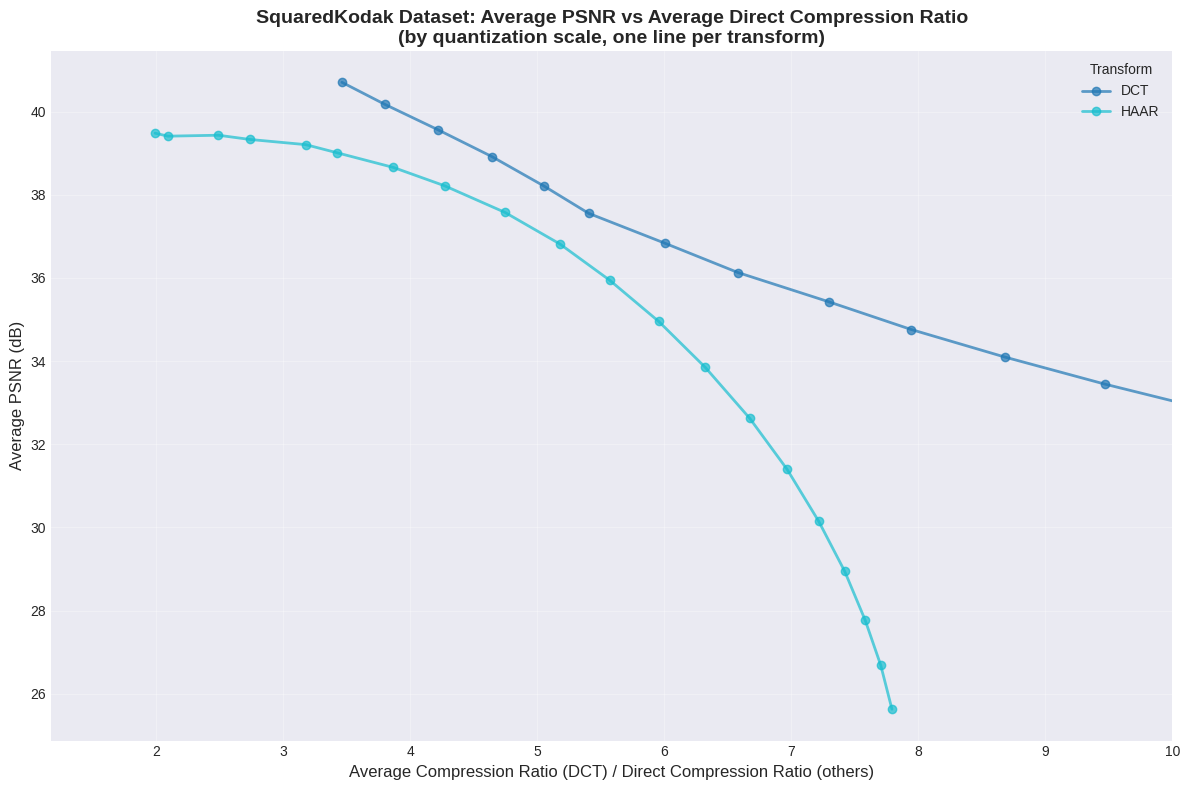
\includegraphics[width=0.48\textwidth]{results/plots/parametric_kodak.png}
  \caption{Performance comparison of Haar and DCT on Kodak images.}
  \label{fig:dwt_kodak}
\end{figure}

In contrast, Figure~\ref{fig:dwt_kodak} demonstrates that Haar performs worse than DCT on Kodak images across all compression ratio scenarios.


\begin{figure}[ht]
  \centering
  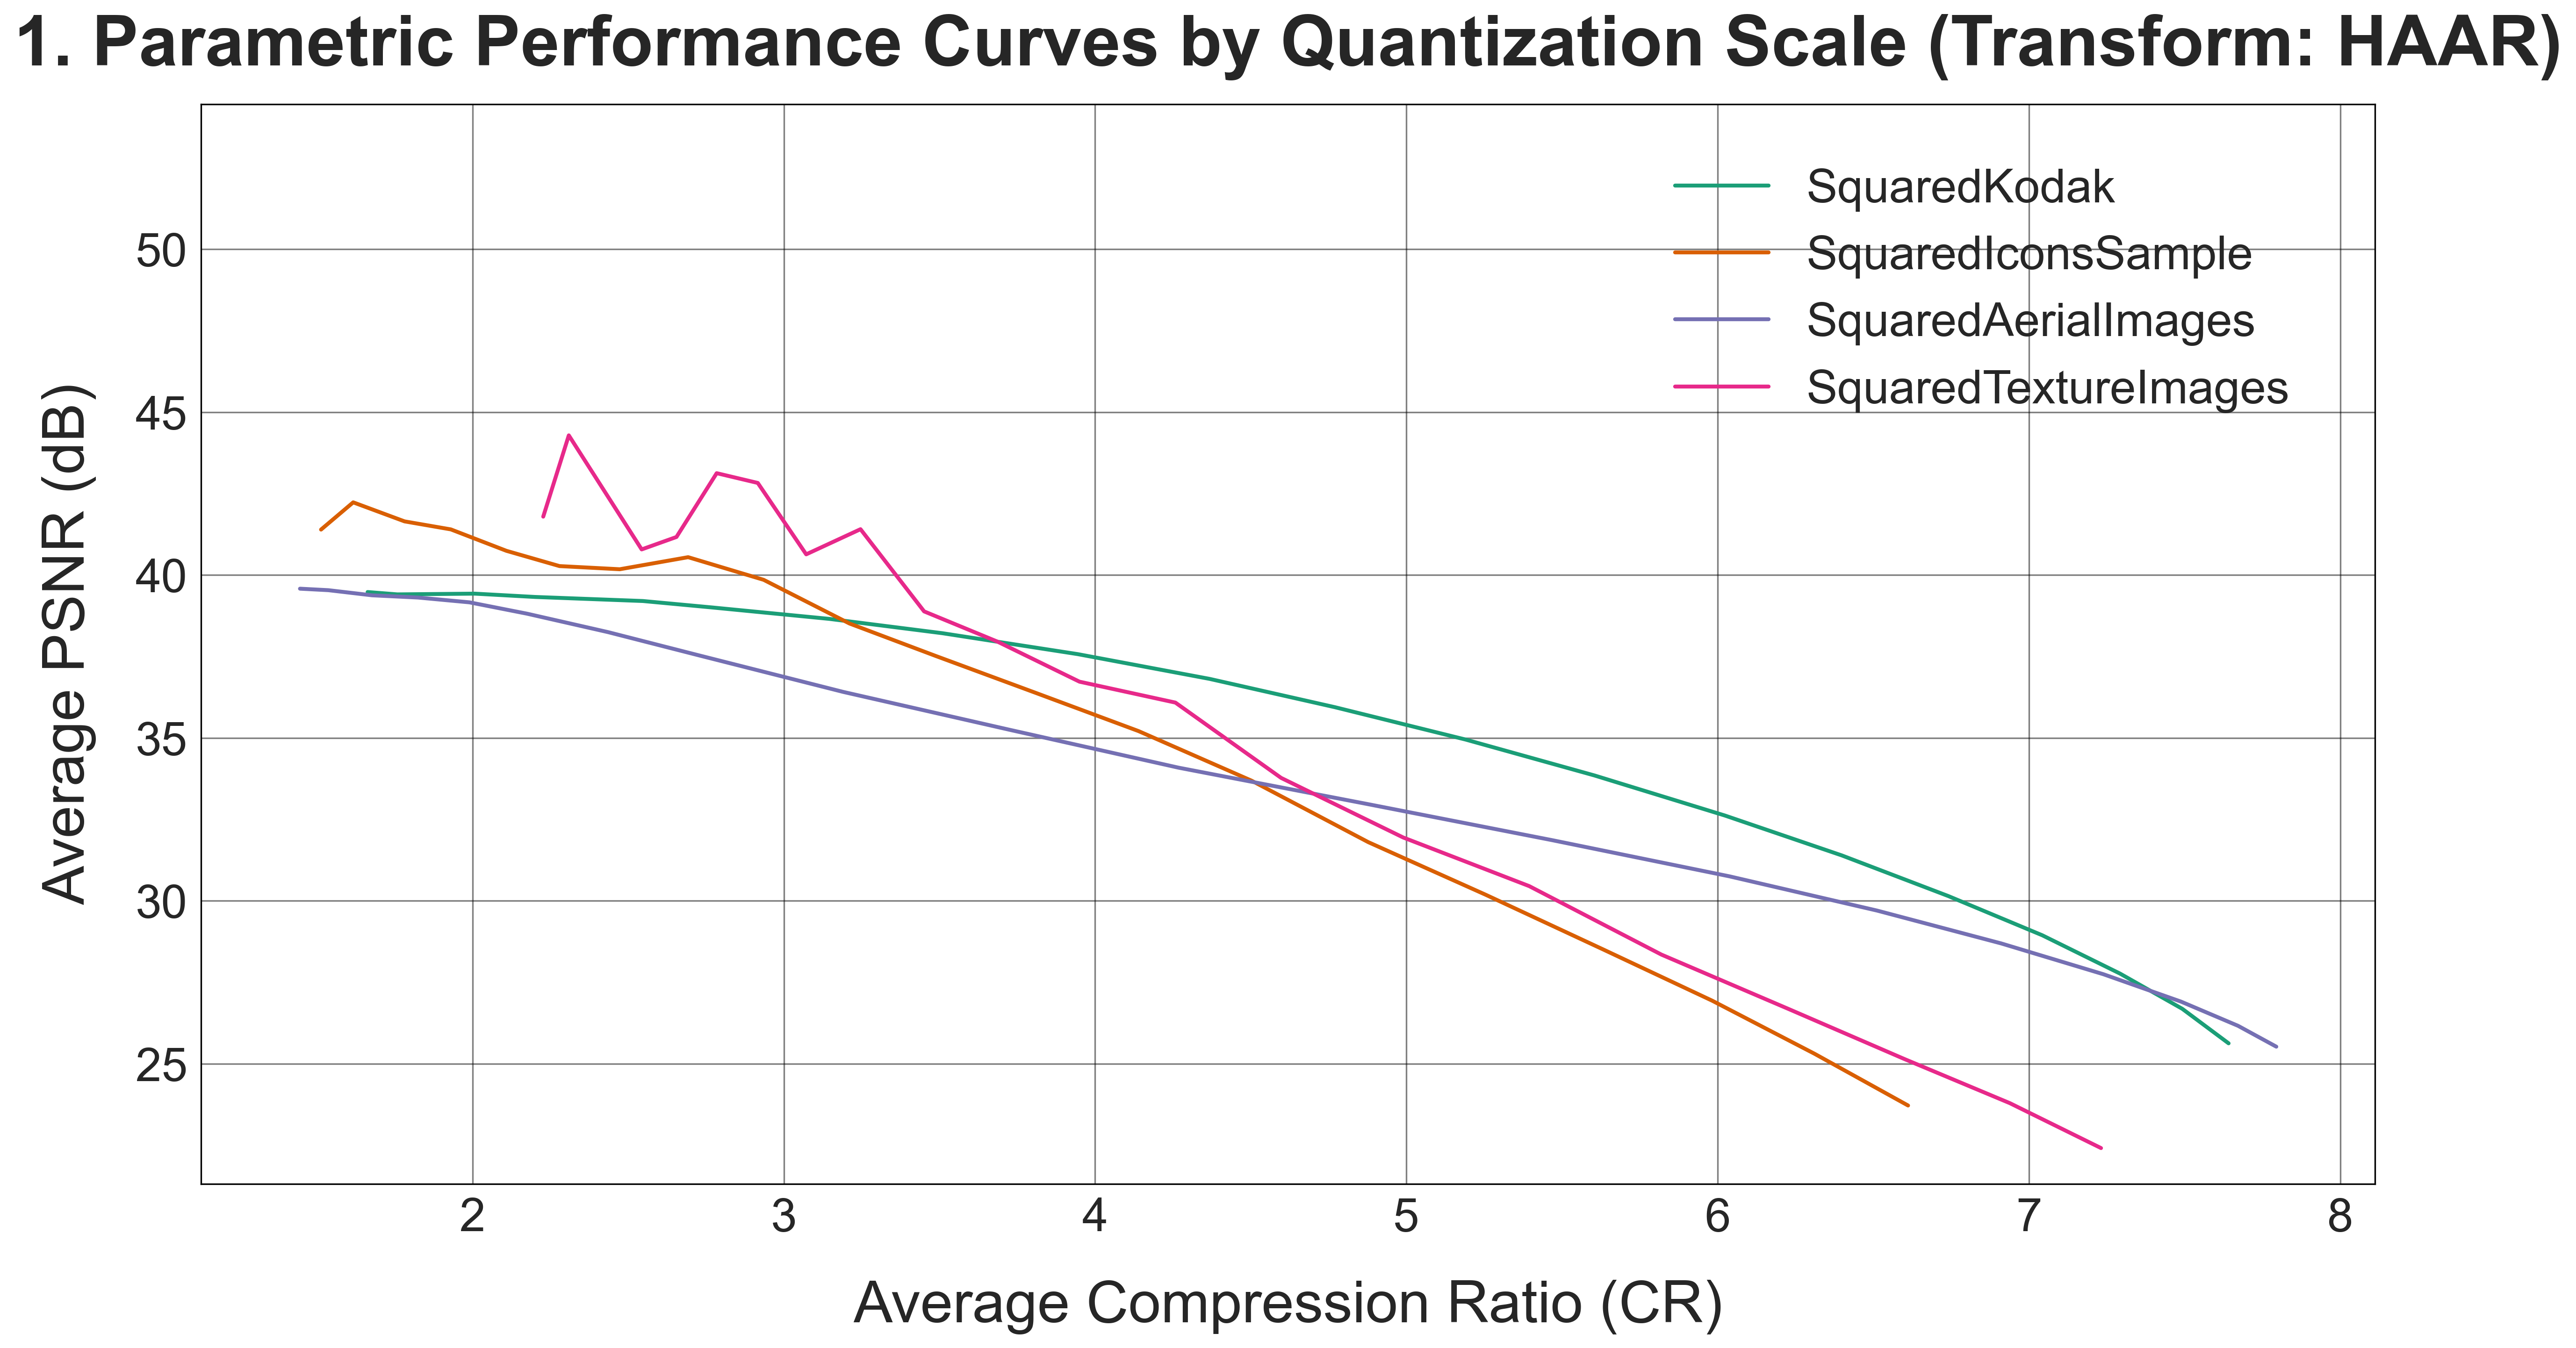
\includegraphics[width=0.48\textwidth]{results/plots/plot_1_parametric_curve_HAAR.png}
  \caption{Performance of the Haar wavelet transform across different datasets}
  \label{fig:dwt_results}
\end{figure}

The results demonstrate that the Discrete Wavelet Transform (DWT) using the Haar wavelet basis exhibits varying performance across different image datasets. Notably, the method performed worse on the Texture Images and Icons Images datasets as quantization became more aggressive compared to other image types as can be see in Figure~\ref{fig:dwt_results}.

\begin{figure}[ht]
  \centering
  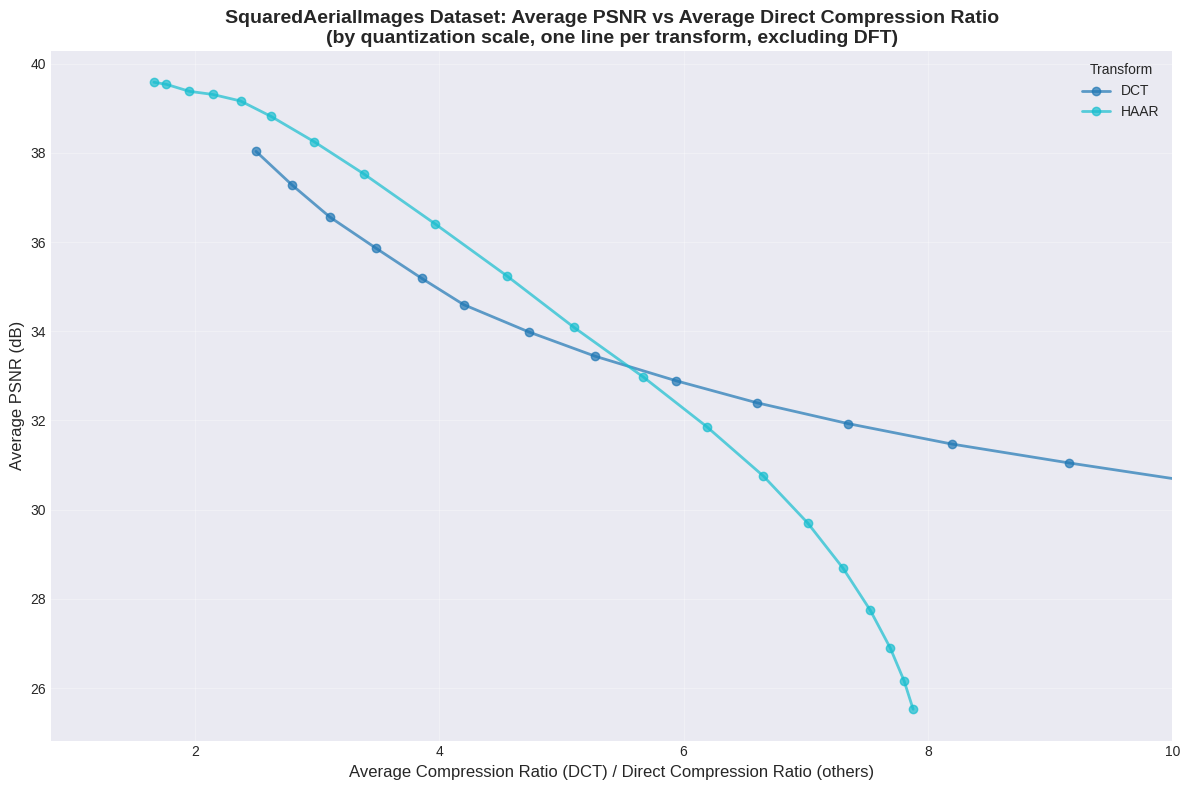
\includegraphics[width=0.48\textwidth]{results/plots/parametric_aerial.png}
  \caption{Performance comparison of Haar and DCT on aerial images.}
  \label{fig:dwt_aerial}
\end{figure}

Figure~\ref{fig:dwt_aerial} shows that the Haar wavelet transform performs slightly better than DCT on aerial images at smaller compression ratios.

\begin{figure}[ht]
  \centering
  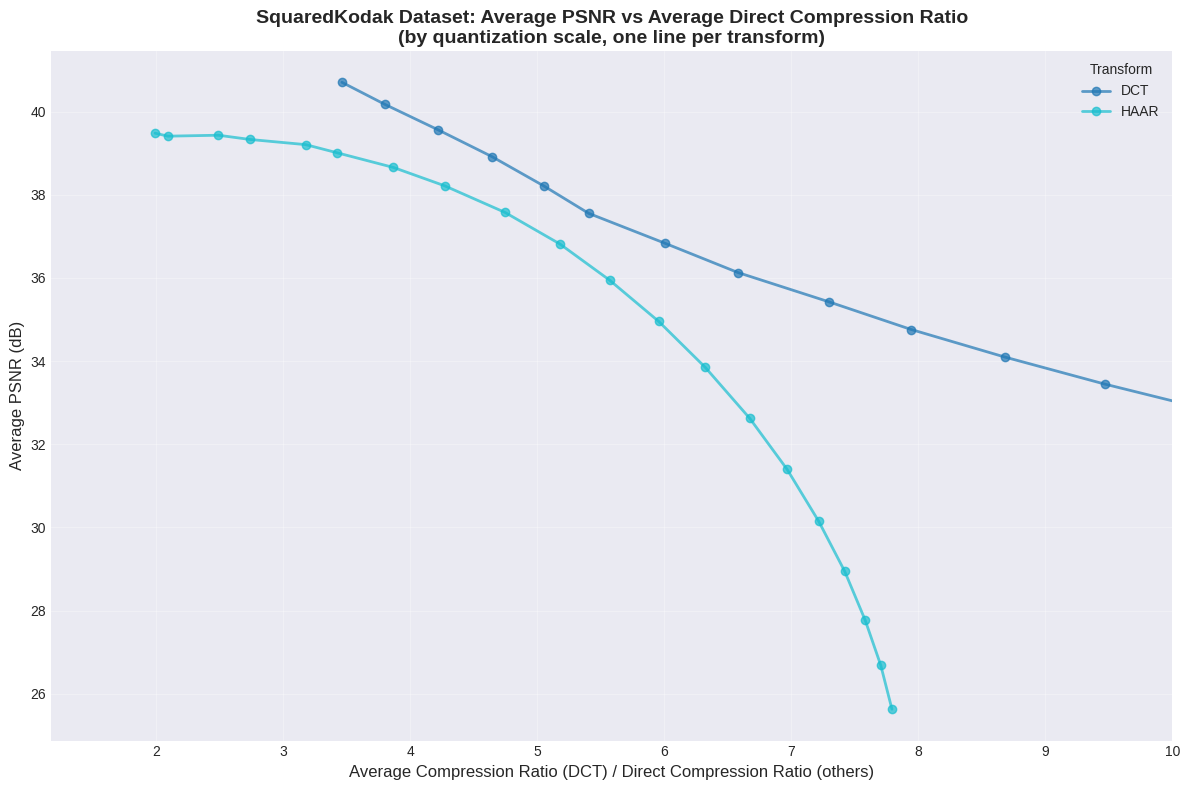
\includegraphics[width=0.48\textwidth]{results/plots/parametric_kodak.png}
  \caption{Performance comparison of Haar and DCT on Kodak images.}
  \label{fig:dwt_kodak}
\end{figure}

In contrast, Figure~\ref{fig:dwt_kodak} demonstrates that Haar performs worse than DCT on Kodak images across all compression ratio scenarios.


\begin{figure}[ht]
  \centering
  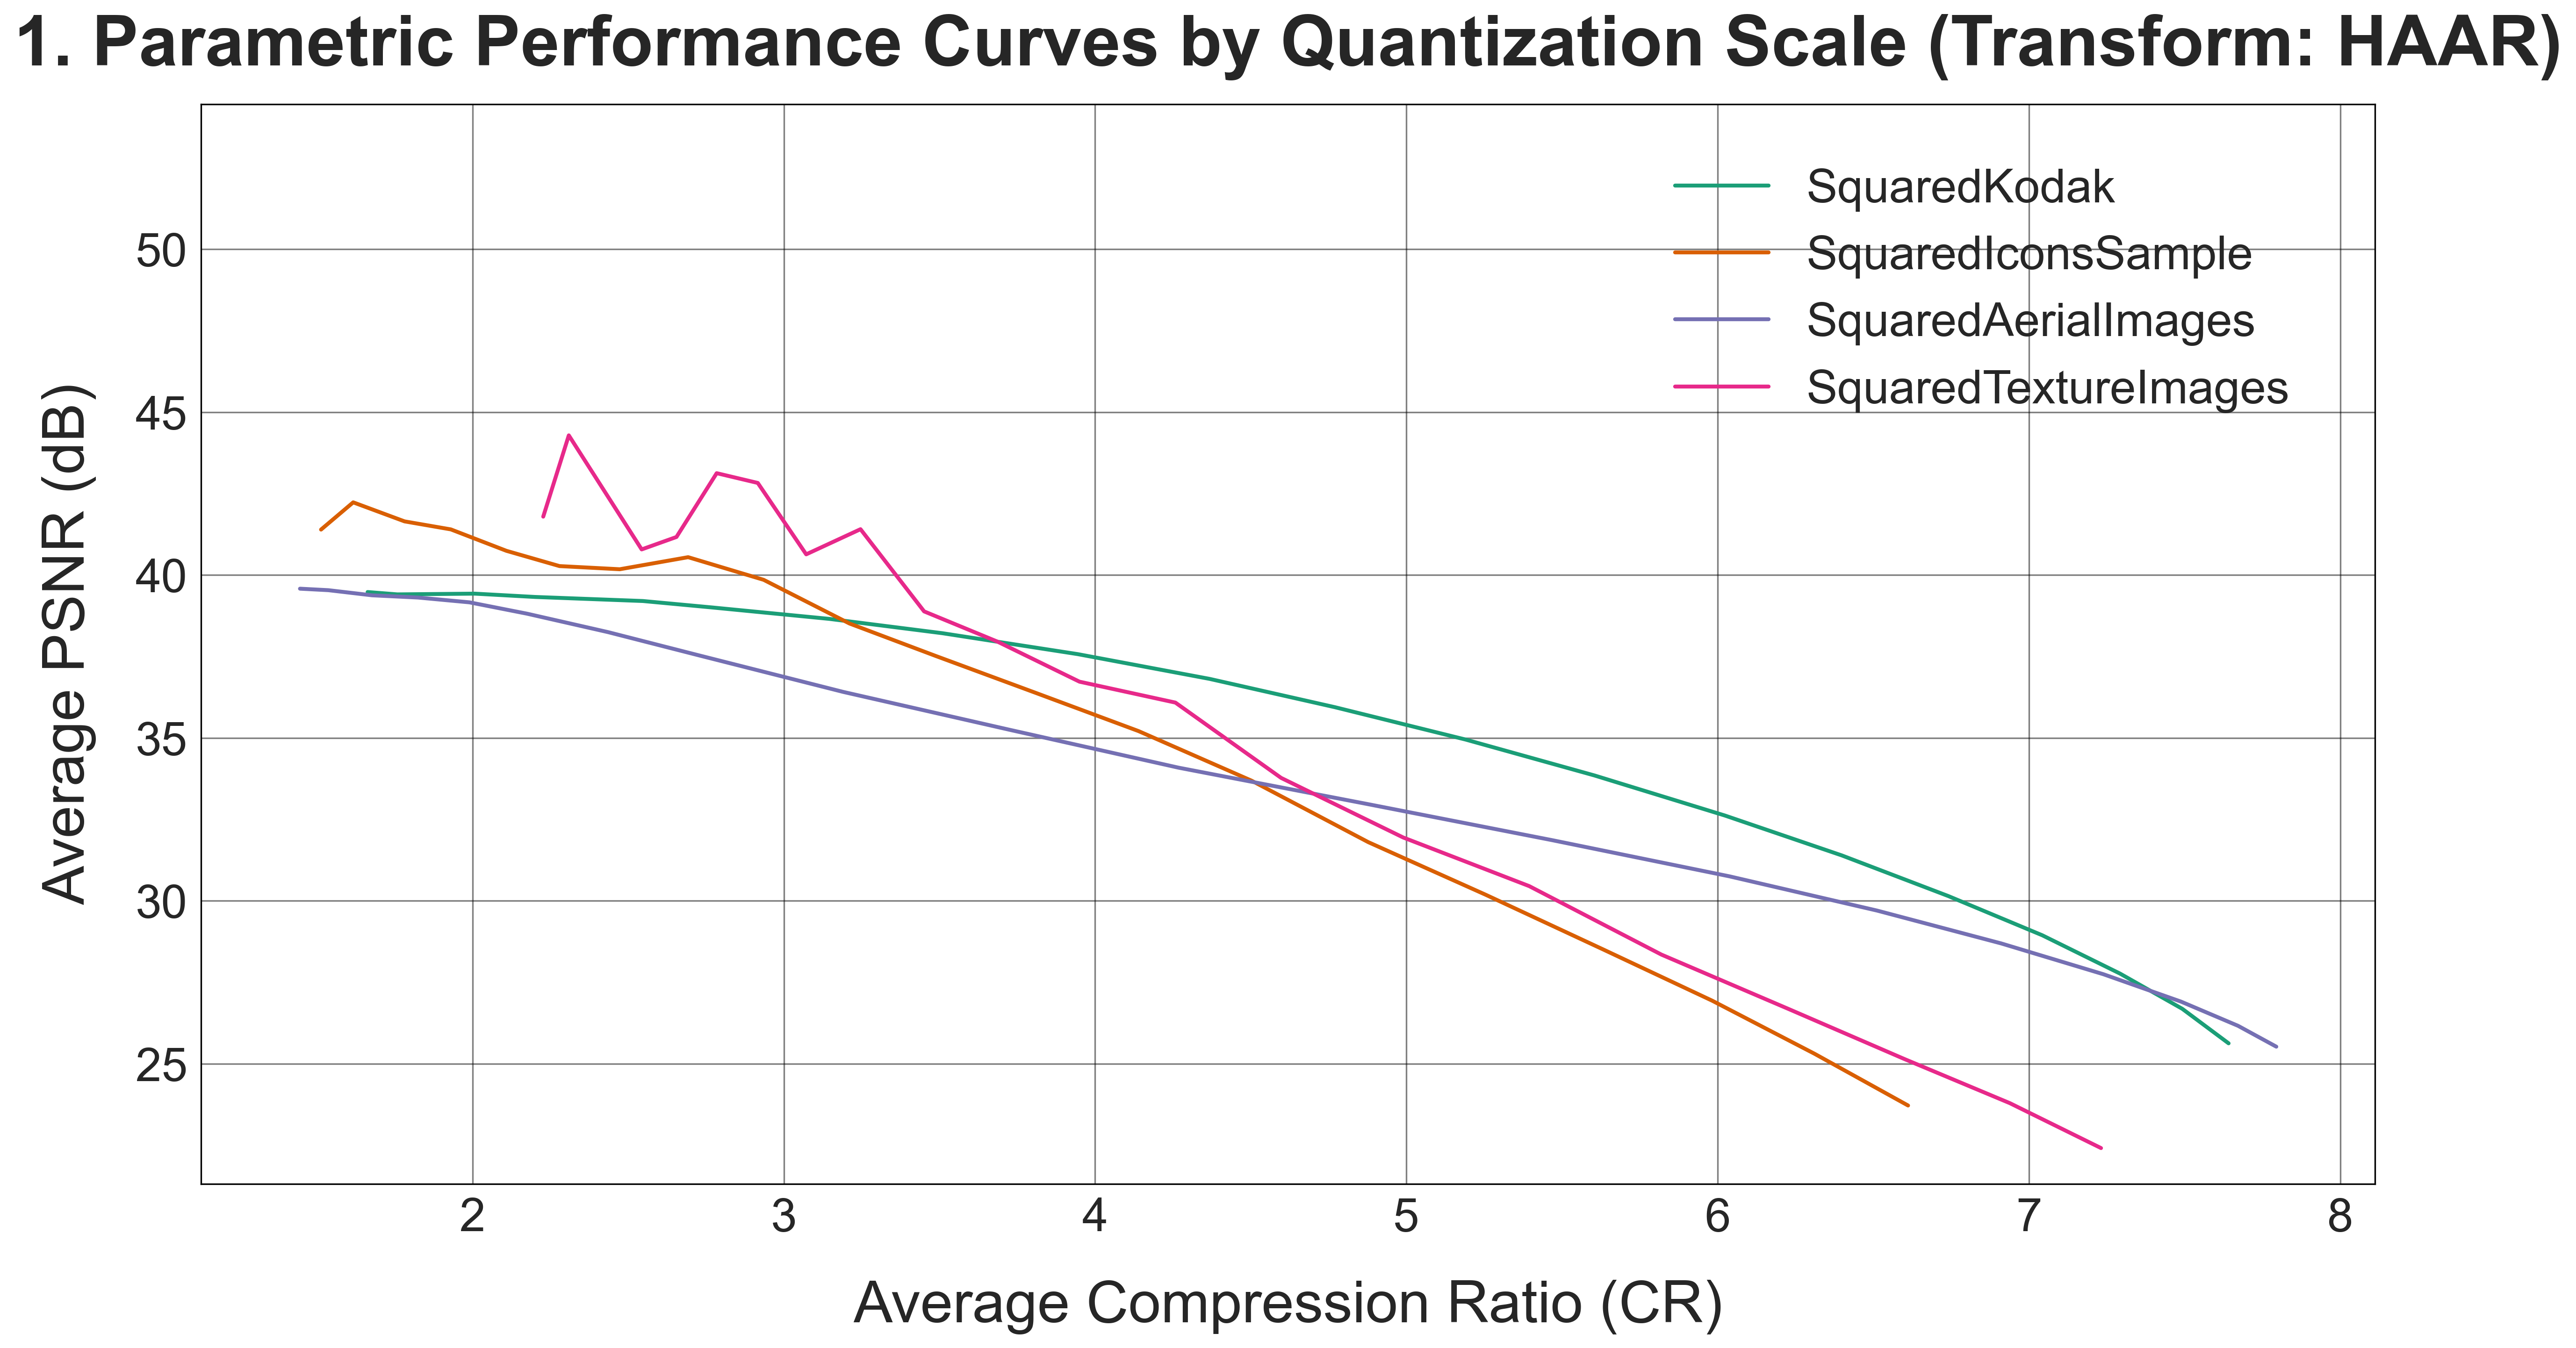
\includegraphics[width=0.48\textwidth]{results/plots/plot_1_parametric_curve_HAAR.png}
  \caption{Performance of the Haar wavelet transform across different datasets}
  \label{fig:dwt_results}
\end{figure}

The results demonstrate that the Discrete Wavelet Transform (DWT) using the Haar wavelet basis exhibits varying performance across different image datasets. Notably, the method performed worse on the Texture Images and Icons Images datasets as quantization became more aggressive compared to other image types as can be see in Figure~\ref{fig:dwt_results}.

\begin{figure}[ht]
  \centering
  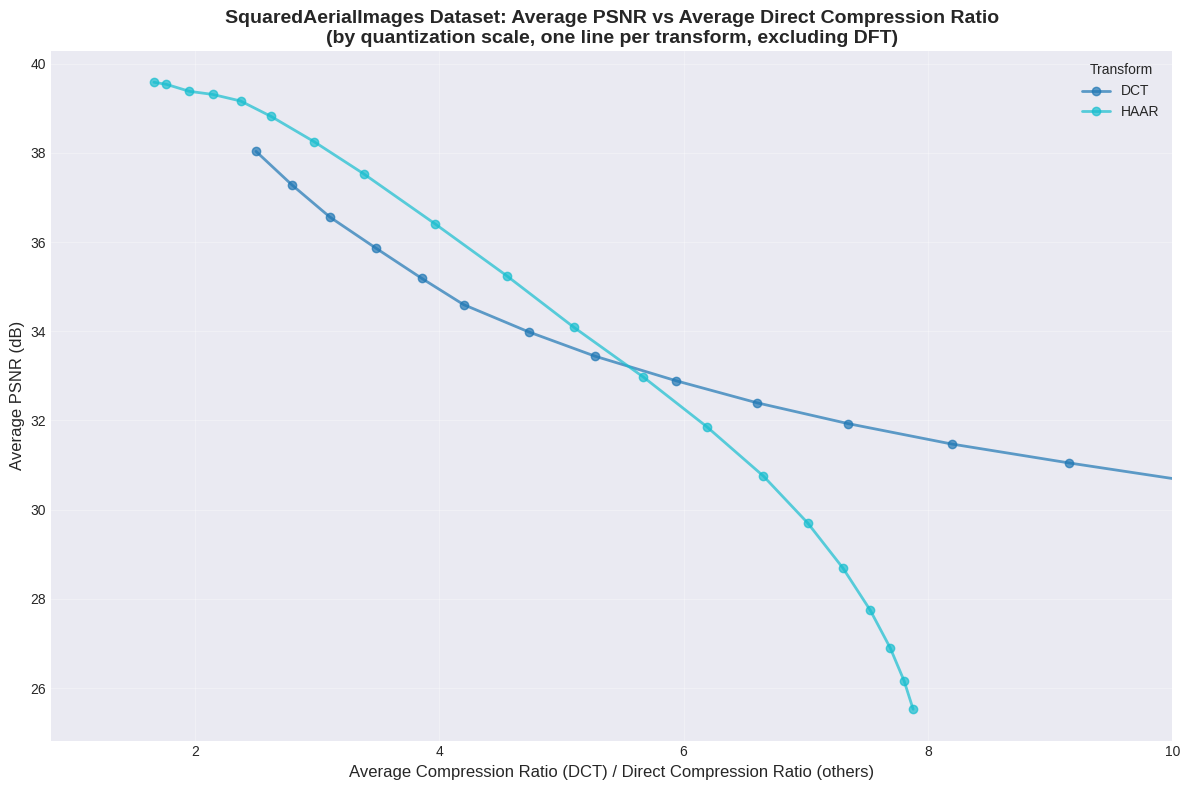
\includegraphics[width=0.48\textwidth]{results/plots/parametric_aerial.png}
  \caption{Performance comparison of Haar and DCT on aerial images.}
  \label{fig:dwt_aerial}
\end{figure}

Figure~\ref{fig:dwt_aerial} shows that the Haar wavelet transform performs slightly better than DCT on aerial images at smaller compression ratios.

\begin{figure}[ht]
  \centering
  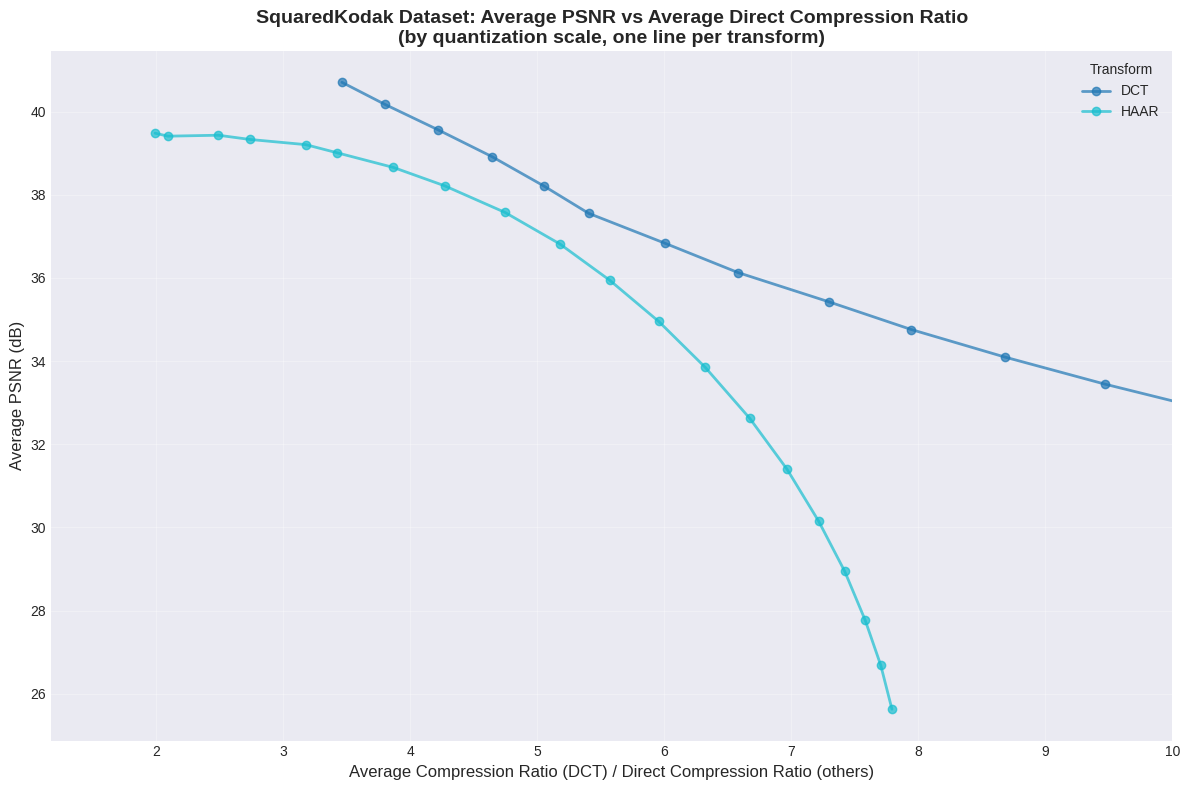
\includegraphics[width=0.48\textwidth]{results/plots/parametric_kodak.png}
  \caption{Performance comparison of Haar and DCT on Kodak images.}
  \label{fig:dwt_kodak}
\end{figure}

In contrast, Figure~\ref{fig:dwt_kodak} demonstrates that Haar performs worse than DCT on Kodak images across all compression ratio scenarios.
